% ============================================================================
%  3. XÂY DỰNG DỮ LIỆU
% ============================================================================
\section{Xây dựng dữ liệu}
\label{sec:du-lieu}

\subsection{Nguồn văn bản và giải trình phạm vi}

Đề bài yêu cầu chọn ``01 văn bản pháp luật tương ứng''. Nhóm thực hiện trên \textbf{bốn}
văn bản và xin giải trình ngay từ đầu, vì đây là quyết định thiết kế chứ không phải làm
lệch đề.

\begin{keybox}
Luật 36/2024/QH15 quy định \textbf{hành vi} nào bị nghiêm cấm nhưng không quy định mức phạt;
toàn bộ \textbf{chế tài} nằm ở Nghị định 168/2024/NĐ-CP. Nếu chỉ dùng văn bản luật gốc, hệ
thống sẽ không trả lời được câu hỏi phổ biến nhất trong thực tế là \emph{``phạt bao nhiêu
tiền''}. Hai văn bản sửa đổi được đưa thêm vào để hệ thống trả lời đúng \textbf{theo mốc thời
gian}, thay vì trả lời theo bản đã lỗi thời.
\end{keybox}

\begin{table}[H]
\centering
\caption{Bốn văn bản nguồn và vai trò trong cơ sở tri thức}
\label{tab:van-ban}
\renewcommand{\arraystretch}{1.2}
\begin{tabularx}{\textwidth}{@{}l L r@{}}
\toprule
\textbf{Văn bản} & \textbf{Vai trò} & \textbf{Hiệu lực} \\
\midrule
Luật 36/2024/QH15~\cite{luat36}        & Văn bản chính --- quy tắc, khái niệm, hành vi bị cấm & 01/01/2025 \\
Nghị định 168/2024/NĐ-CP~\cite{nd168}  & Văn bản chế tài --- mức phạt, trừ điểm GPLX          & 01/01/2025 \\
Luật 118/2025/QH15~\cite{luat118}      & Sửa đổi Luật 36/2024                                  & 01/7/2026 \\
Nghị định 238/2026/NĐ-CP~\cite{nd238}  & Sửa đổi Nghị định 168/2024                            & 15/8/2026 \\
\bottomrule
\end{tabularx}
\end{table}

Mọi mục tri thức đều được đối chiếu với Văn bản hợp nhất 55/VBHN-VPQH ngày
23/3/2026~\cite{vbhn55} của Văn phòng Quốc hội --- tức bản \emph{sau} sửa đổi. Trường
\code{can\_cu\_text} của từng bản ghi ghi rõ điều này, nên người chấm kiểm tra được ngay rằng
dữ liệu không phải bản cũ.

\subsection{Cấu trúc của cơ sở tri thức}

\begin{table}[H]
\centering
\caption{Năm thành phần của cơ sở tri thức $K$}
\label{tab:thanh-phan-K}
\renewcommand{\arraystretch}{1.2}
\begin{tabularx}{\textwidth}{@{}c l r L@{}}
\toprule
\textbf{Ký hiệu} & \textbf{Thành phần} & \textbf{Số lượng} & \textbf{Vai trò} \\
\midrule
$C$                 & Khái niệm        & 73    & Định nghĩa pháp lý --- ``xe cơ giới là gì'' \\
$R$                 & Quan hệ          & 482   & Đồ thị hai chiều nối các mảng tri thức \\
$\mathit{Rules}$    & Quy tắc          & 109   & Quy định phải làm / không được làm \\
$F$                 & Hành vi vi phạm  & 345   & Hành vi kèm chế tài: tiền, trừ điểm, hình phạt bổ sung \\
$\mathit{Keyphrase}$& Cụm từ khoá      & 1.674 & Cầu nối giữa ngôn ngữ người dùng và định danh tri thức \\
\bottomrule
\end{tabularx}
\end{table}

Ngoài năm thành phần trên, cơ sở tri thức còn lưu 4 bản ghi văn bản nguồn và \textbf{63 bản
ghi sửa đổi}. Sửa đổi được lưu như dữ liệu độc lập, không hợp nhất cứng lúc dựng cơ sở tri
thức --- nhờ vậy hệ thống trả lời được câu hỏi ``tại thời điểm nào thì quy định ra sao''.

\subsection{Cách lấy và chuẩn hoá dữ liệu}

\begin{itemize}
  \item \textbf{Trích xuất:} tách toàn văn theo cấu trúc điều -- khoản -- điểm từ bản công bố
        của bốn văn bản, lưu ở \code{data/raw/} dưới dạng JSON giữ nguyên văn. Không dùng bản
        tóm tắt hay bài viết lại của bên thứ ba.
  \item \textbf{Chuẩn hoá:} mỗi mục tri thức được gán một định danh ổn định (ví dụ
        \code{R01}, \code{VP\_OTO\_ND168D6\_K1A}), một khối căn cứ có cấu trúc và một khoảng
        hiệu lực. Chế tài được lưu \emph{có kiểu} --- số tiền và điểm trừ là số nguyên, không
        phải chuỗi --- nên cộng dồn và so sánh được.
  \item \textbf{Sinh keyphrase:} mỗi mục kèm danh sách cụm từ người dùng thật hay dùng, gồm
        cả khẩu ngữ (``nhậu'', ``vượt đèn đỏ'') và bản không dấu, để chịu được truy vấn gõ vội
        không dấu.
  \item \textbf{Kiểm toàn vẹn:} module \code{kb/validator.py} soát định danh trùng, quan hệ
        treo, keyphrase trỏ tới định danh không tồn tại và mục thiếu căn cứ. Toàn bộ kiểm tra
        này chạy trong CI, nên một bản ghi hỏng không thể lọt vào kho mã.
  \item \textbf{Xây bộ câu hỏi đánh giá:} mỗi câu được viết kèm đáp án chuẩn dạng văn bản,
        danh sách \emph{định danh} tri thức đúng, lớp bài toán đúng và mức độ khó. Có test kiểm
        chứng rằng mọi định danh trong đáp án chuẩn đều tồn tại trong cơ sở tri thức --- hiện
        120/120 câu đều chấm được, không có định danh treo.
\end{itemize}

Chuẩn hoá bằng mô hình có kiểu (Pydantic v2) chứ không phải \code{dict} tự do: trường lạ bị
từ chối ngay lúc nạp, nên một bản ghi sai cấu trúc không thể lọt vào cơ sở tri thức để đến
lúc chạy mới phát hiện. Một bản ghi hành vi vi phạm (rút gọn):

\begin{lstlisting}
{
  "id": "VP_OTO_ND168D6_K1A",
  "hanh_vi": "Không chấp hành hiệu lệnh, chỉ dẫn của biển báo hiệu,
              vạch kẻ đường, trừ ...",
  "nhom": "bien_bao_hieu",
  "phuong_tien": ["o_to"],
  "phat_tien": { "min": 400000, "max": 600000 },
  "tru_diem_gplx": 0,
  "can_cu": { "van_ban": "Nghị định 168/2024/NĐ-CP",
              "dieu": 6, "khoan": 1, "diem": "a" },
  "tinh_trang": "hien_hanh"
}
\end{lstlisting}

\subsection{Thống kê và phân tích bộ dữ liệu}

Ba phân bố dưới đây được sinh lại bằng một lệnh (xem Phụ lục~B) nên luôn khớp với dữ liệu thật trong kho mã, không phải số chép tay.

\subsubsection{Phân bố độ dài}

Câu hỏi dài trung bình \textbf{14,61 từ} (trung vị 14, ngắn nhất 3, dài nhất 38, độ lệch
chuẩn 6,10). Phân bố lệch phải rõ rệt: 75\% câu không quá 17 từ, nhưng đuôi kéo tới 38 từ --- đó
là các câu khẩu ngữ kể cả tình huống (\emph{``Nhóm em 4 đứa đi chung một xe máy, không ai đội
mũ bảo hiểm\dots''}). Đuôi này quan trọng: mục~\ref{sec:ket-qua} sẽ cho thấy phần lớn ca lỗi
nặng tập trung ở đó.

Về phía tri thức, hành vi vi phạm dài trung bình 42,0 từ và quy tắc dài trung bình 80,8 từ
--- dài gấp khoảng 5,5 lần câu hỏi. Đây là gốc rễ của bài toán: câu hỏi ngắn và đời thường
phải khớp với văn bản dài và trang trọng, nên chỉ so khớp bề mặt là không đủ.

\begin{figure}[H]
\centering
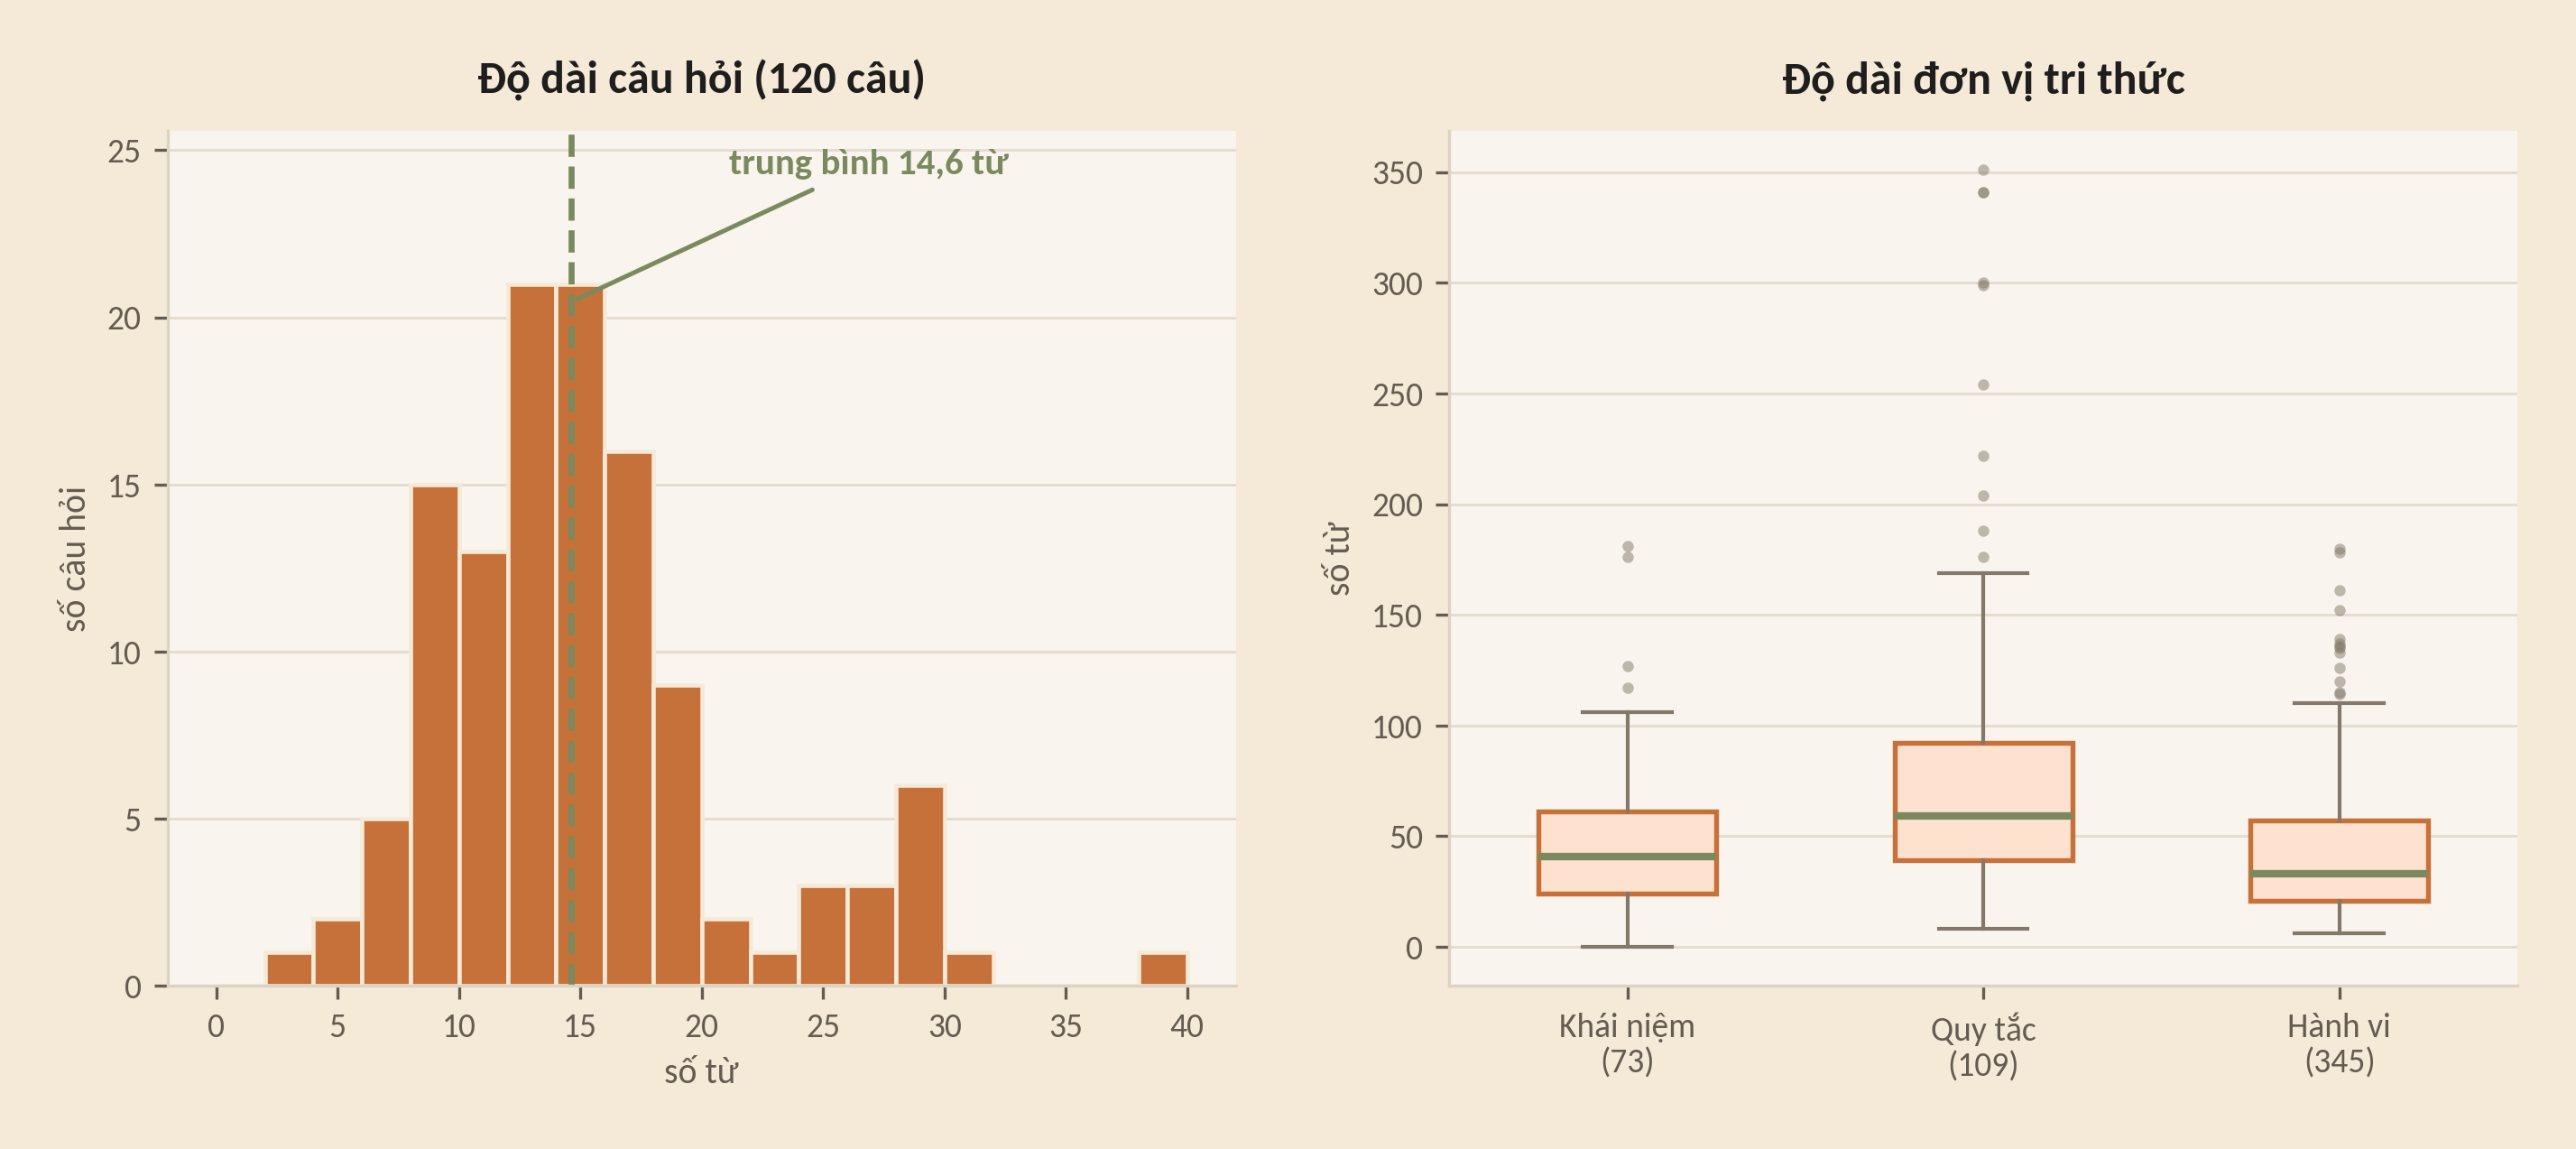
\includegraphics[width=\textwidth]{figures/hinh3_phan_bo_do_dai.png}
\caption{Phân bố độ dài câu hỏi và độ dài đơn vị tri thức}
\label{fig:do-dai}
\end{figure}

\subsubsection{Phân bố nhãn}

Bộ câu hỏi được phân bổ theo tần suất thực tế của nhu cầu tra cứu, không chia đều: lớp tra
cứu chế tài P3 chiếm 40/120 câu vì đây là câu hỏi người dân hỏi nhiều nhất. Về mức độ khó:
dễ 28 · trung bình 68 · khó 24. Về loại tri thức của đáp án chuẩn: khái niệm 22 · quy tắc 25
· hành vi vi phạm 73. Có \textbf{26/120 câu} có nhiều hơn một mẩu tri thức trong đáp án chuẩn
--- chi tiết này sẽ giải thích con số precision ở mục~\ref{sec:kiem-dinh}.

\begin{figure}[H]
\centering
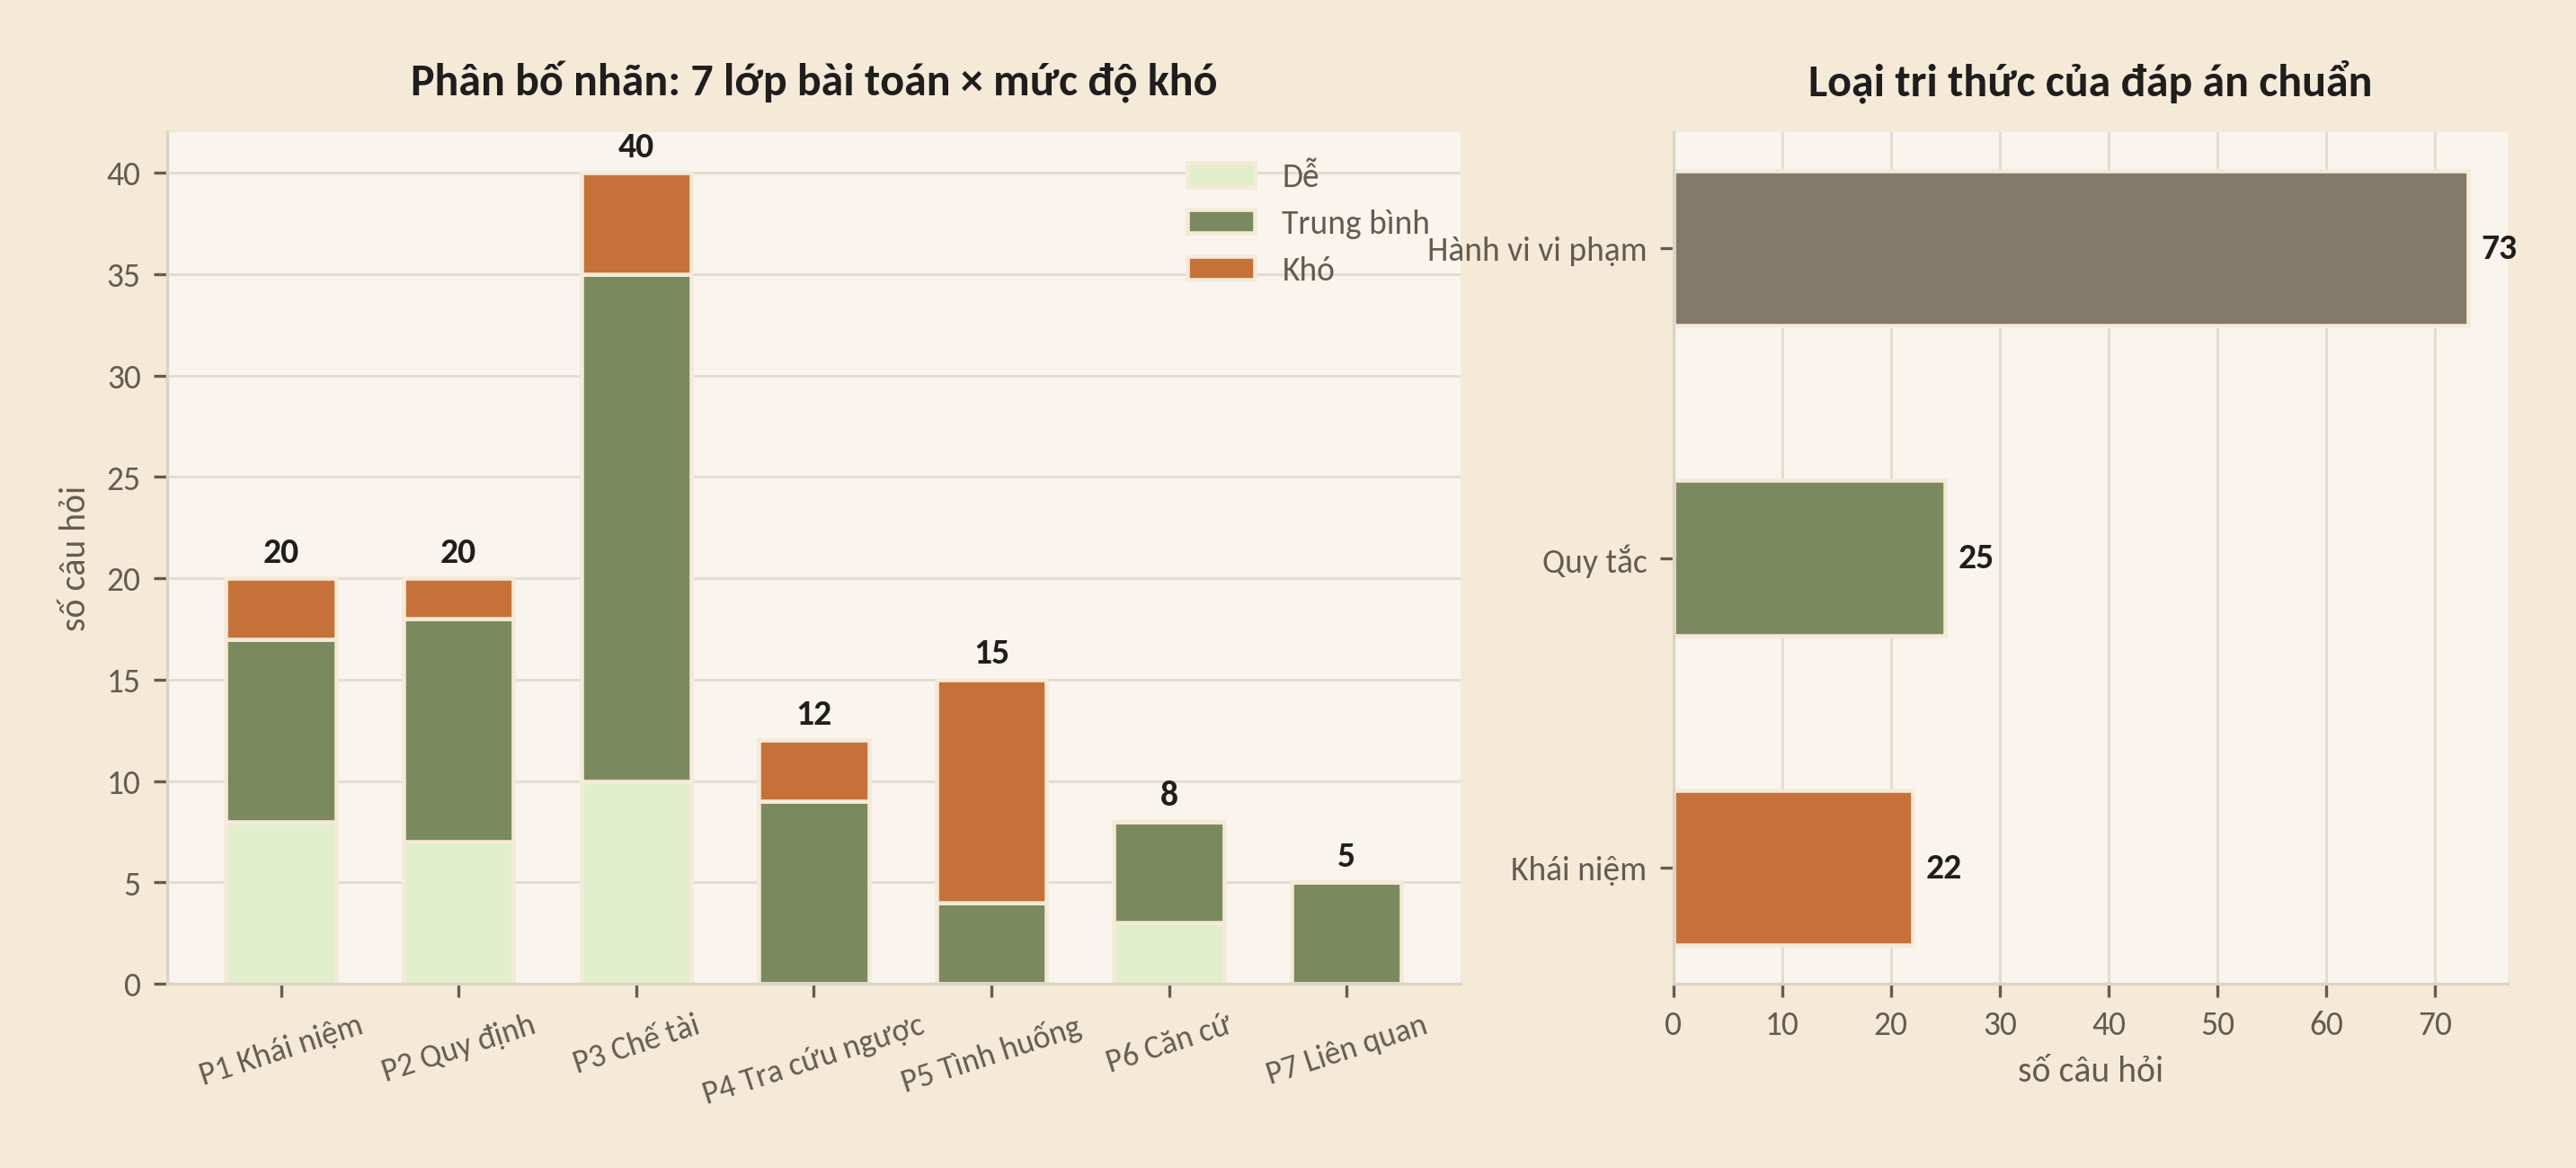
\includegraphics[width=\textwidth]{figures/hinh4_phan_bo_nhan.png}
\caption{Phân bố nhãn của bộ câu hỏi có đáp án chuẩn}
\label{fig:nhan}
\end{figure}

\subsubsection{Phân bố chủ đề}

Cơ sở tri thức chia thành 6 lĩnh vực và 55 nhóm hành vi. Tỉ trọng trong cơ sở tri thức và
trong bộ câu hỏi \emph{không} trùng nhau, và đây là chủ ý: lĩnh vực ``An toàn của người tham
gia giao thông'' chiếm 19\% cơ sở tri thức nhưng 43\% bộ câu hỏi, vì nồng độ cồn và mũ bảo
hiểm là hai chủ đề được hỏi nhiều nhất ngoài đời. Ngược lại, ``Điều kiện của phương tiện''
chiếm 17\% cơ sở tri thức nhưng chỉ 8\% bộ câu hỏi.

\begin{warnbox}
Nhóm ghi nhận đây là một \textbf{hạn chế của bộ đánh giá} chứ không giấu đi: bộ câu hỏi phản
ánh nhu cầu tra cứu phổ biến, nên chưa phủ đều mọi ngóc ngách của cơ sở tri thức --- tính
theo định danh, 120 câu mới chạm tới 115/527 mục tri thức truy hồi được (21,8\%). Một bộ đánh
giá phủ đều hơn là việc cần làm tiếp, nêu ở mục~\ref{sec:huong-phat-trien}.
\end{warnbox}

\begin{figure}[H]
\centering
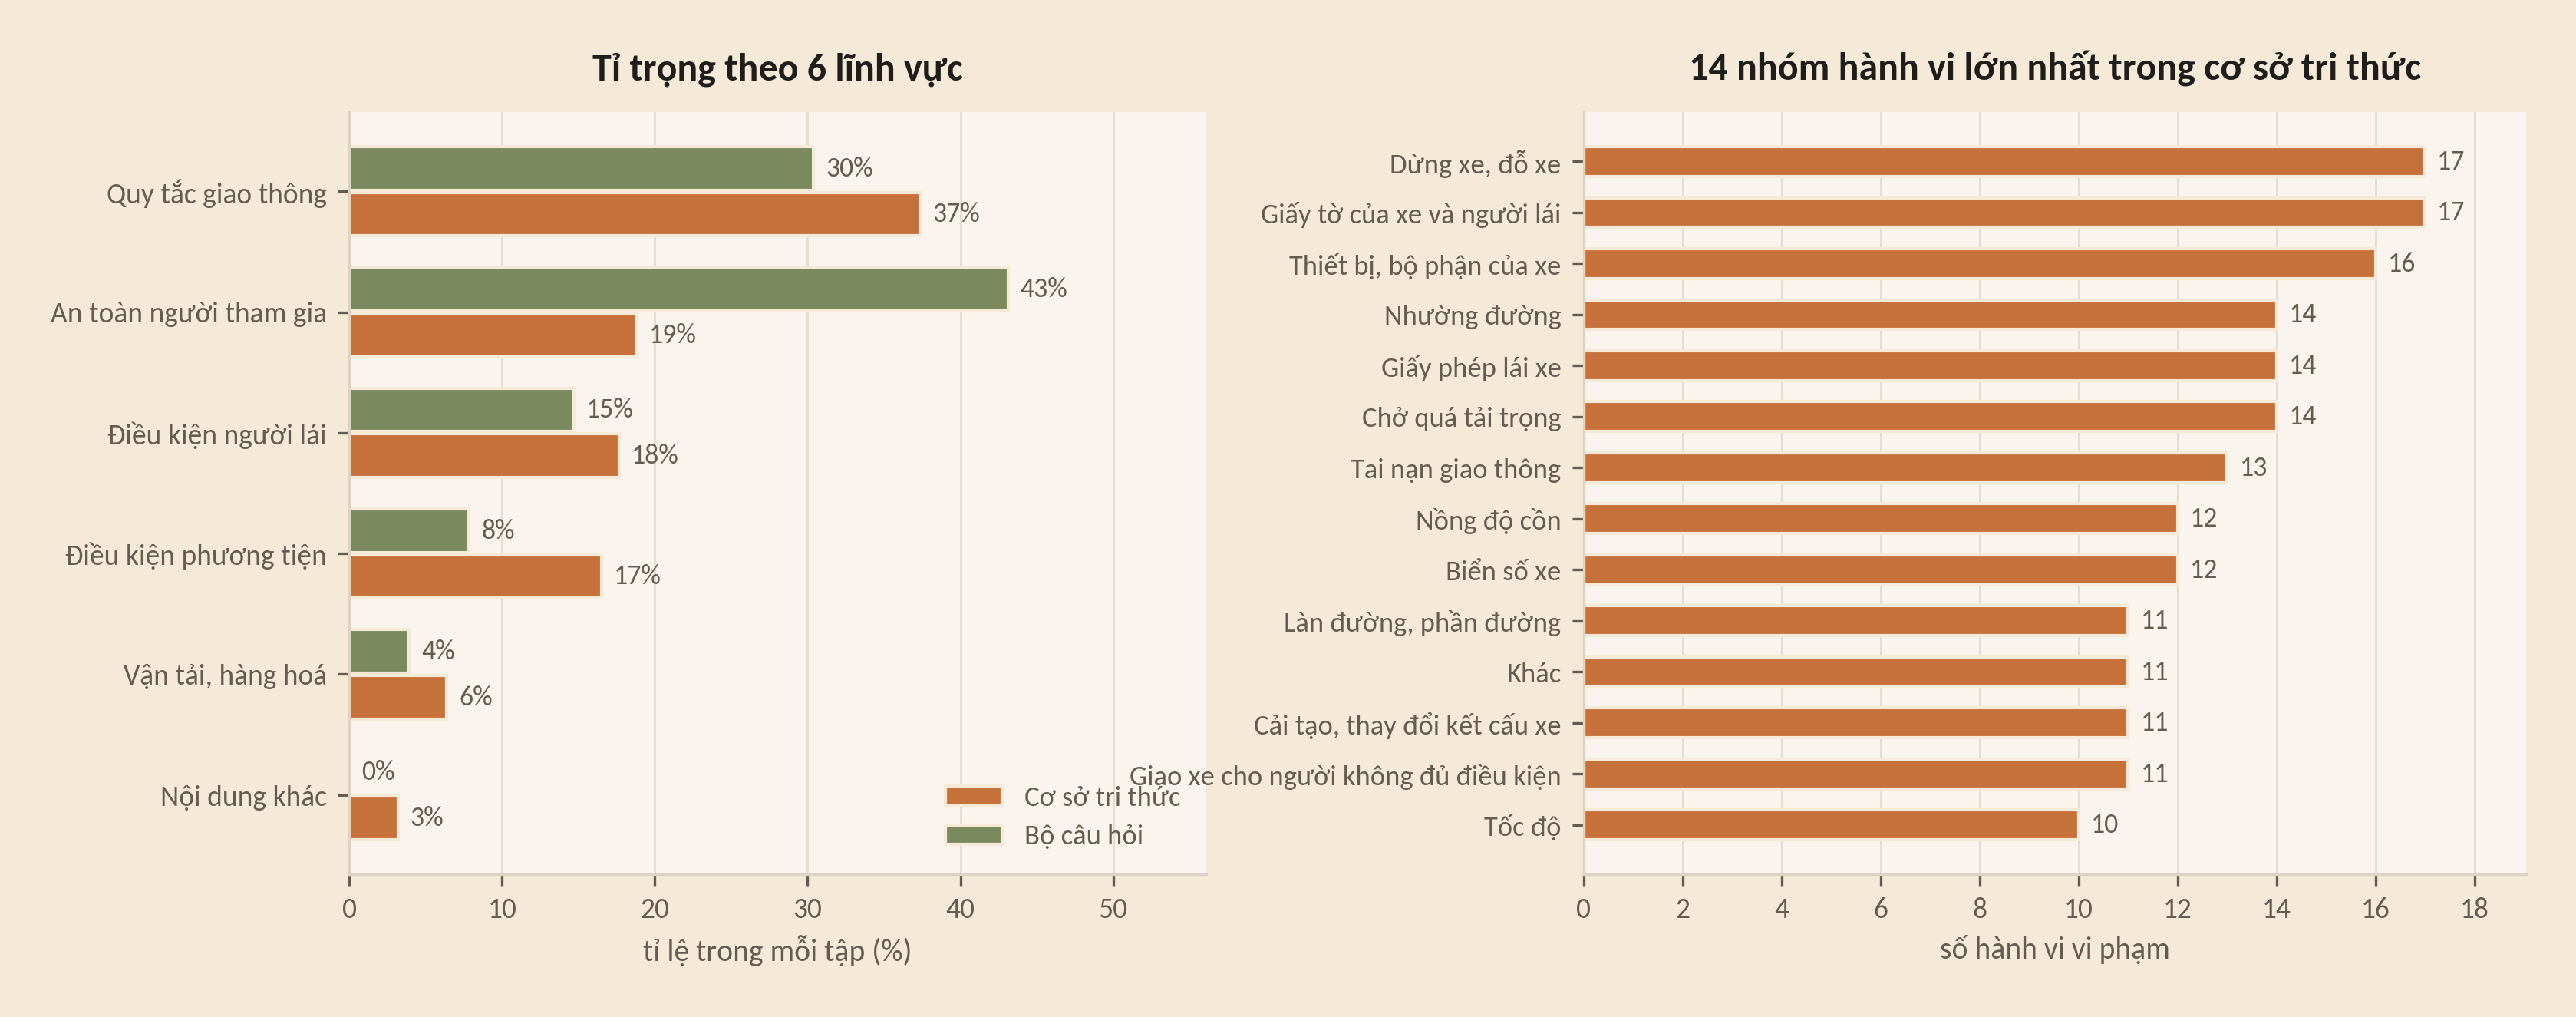
\includegraphics[width=\textwidth]{figures/hinh5_phan_bo_chu_de.png}
\caption{Phân bố chủ đề --- tỉ trọng lĩnh vực và nhóm hành vi}
\label{fig:chu-de}
\end{figure}
